
\section{Thực nghiệm}

\subsection{Huấn luyện}

Trong thiết lập thực nghiệm baseline, tập \texttt{test} của bộ \texttt{FoodSeg103} được giữ nguyên để làm tập đánh giá cuối cùng, gồm 2{,}135 ảnh. Từ tập \texttt{train} gốc, dữ liệu được chia tiếp thành tập huấn luyện và tập kiểm định nội bộ theo tỉ lệ 90/10 bằng hàm \texttt{train\_test\_split} với \texttt{random\_state} cố định theo seed của thí nghiệm. Cách chia này giúp tách rõ ba vai trò: \texttt{train} để tối ưu tham số, \texttt{validation} để theo dõi hội tụ và chọn checkpoint, còn \texttt{test} giữ nguyên như tập đánh giá độc lập.

% Bảng 1: Cấu hình huấn luyện
\begin{table}[H]
    \centering
    \caption{Cấu hình tham số huấn luyện mô hình cơ sở BiSeNet.}
    \label{tab:bisenet-baseline-config}
    \resizebox{\columnwidth}{!}{%
    \begin{tabular}{ll}
        \toprule
        \textbf{Tham số (Hyperparameter)} & \textbf{Giá trị / Thiết lập} \\
        \midrule
        Kích thước crop đầu vào (Crop size) & $512 \times 512$ \\
        Kiến trúc mạng xương sống (Backbone) & Xception39 \\
        Hàm tối ưu (Optimizer) & SGD (Momentum = 0.9, Weight decay = $1\times10^{-4}$) \\
        Hàm mất mát (Loss function) & Cross-Entropy, auxiliary weight = 1.0 \\
        Tốc độ học khởi tạo (Initial LR) & $2.5\times10^{-2}$ với chiến lược Poly (power = 0.9) \\
        Kích thước lô (Batch size) & 8 \\
        Số epoch huấn luyện (Epochs) & 150 \\
        Tỉ lệ validation (Val ratio) & 0.1 \\
        Data augmentation scale & $\{0.75, 1.0, 1.5, 1.75, 2.0\}$ \\
        Số worker nạp dữ liệu (Num workers) & 0 \\
        Ignore index & 255 \\
        Automatic Mixed Precision (AMP) & True \\
        Resume training & True \\
        \bottomrule
    \end{tabular}}
\end{table}

\subsection{Kết quả}

Hình \ref{fig:bisenet-train-val-loss} và Hình \ref{fig:bisenet-val-metrics} trình bày diễn biến huấn luyện của BiSeNet trên bộ \texttt{FoodSeg103} nguyên thủy. Loss huấn luyện và loss kiểm định cùng giảm theo epoch và dần ổn định ở giai đoạn cuối. Đồng thời, các chỉ số đánh giá trên tập validation (\texttt{mIoU}, \texttt{mAcc}, \texttt{aAcc}) tăng đều theo quá trình học, cho thấy mô hình hội tụ theo hướng tích cực.

\begin{figure}[H]
    \centering
    \begin{subfigure}{0.49\linewidth}
        \centering
        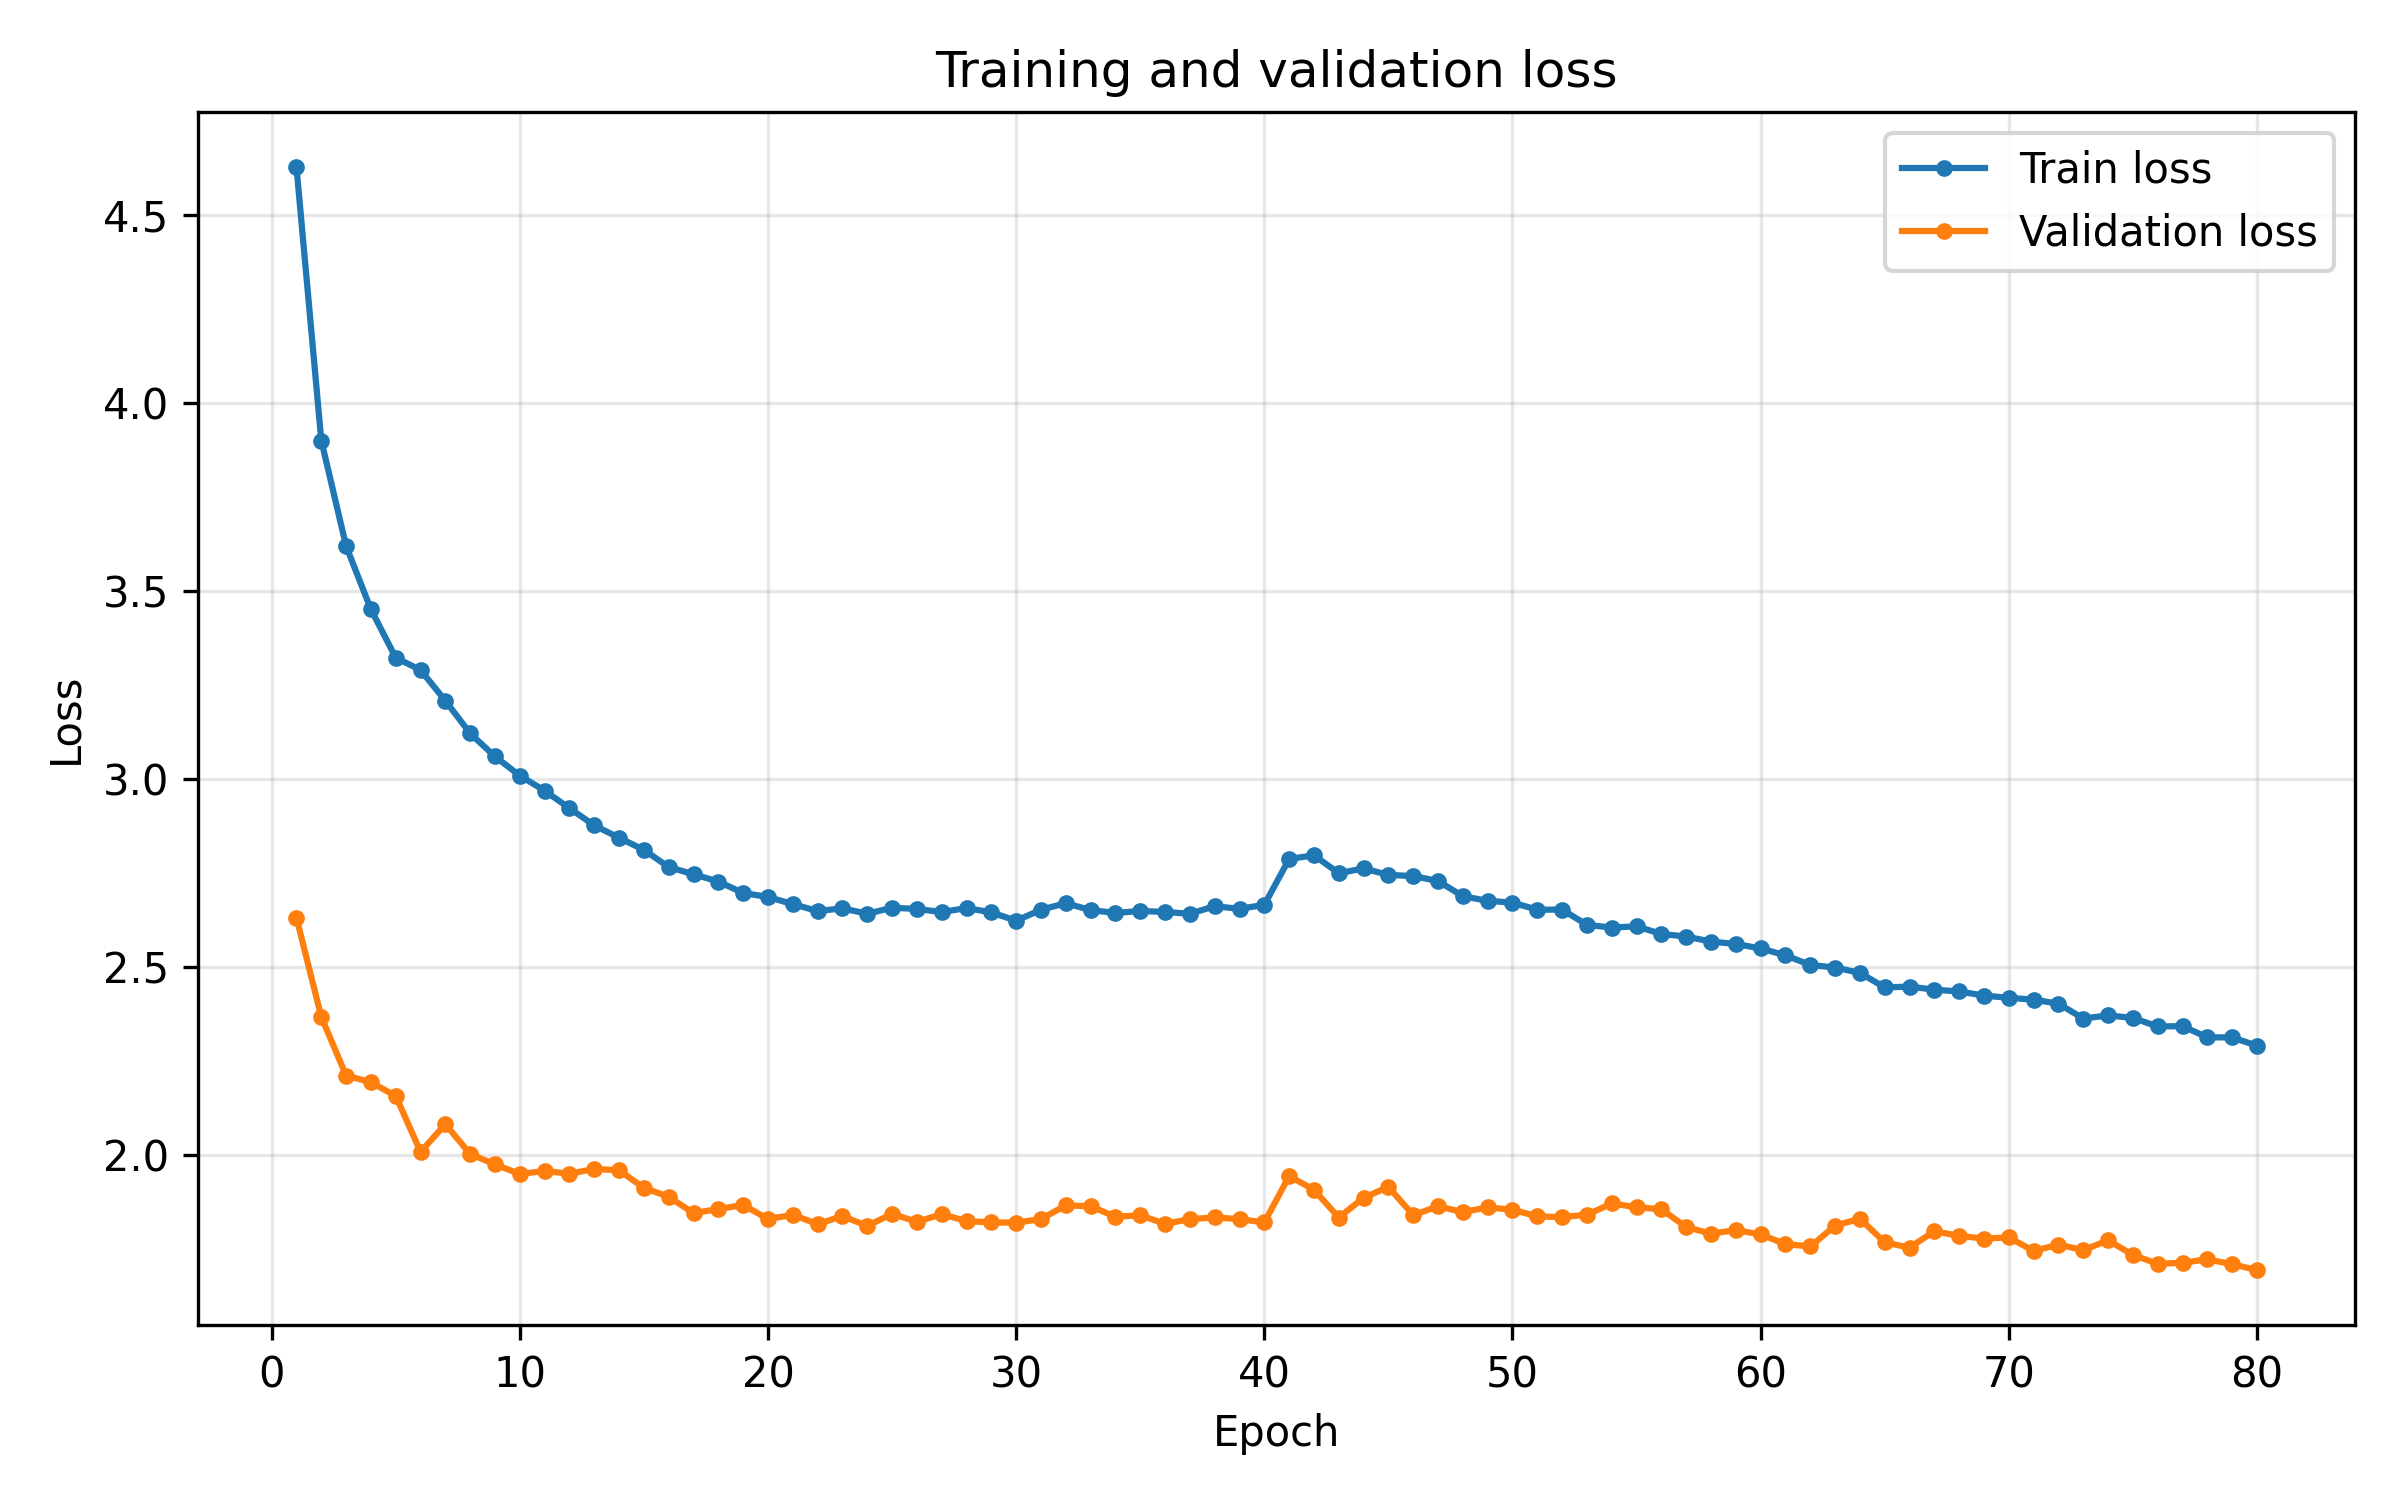
\includegraphics[width=\linewidth]{img/outputs/loss_curve.png}
        \caption{Train loss và validation loss.}
        \label{fig:bisenet-train-val-loss}
    \end{subfigure}
    \hfill
    \begin{subfigure}{0.49\linewidth}
        \centering
        
\includegraphics[width=\linewidth]{img/outputs/metrics_curve.png}
        \caption{Các chỉ số validation: \texttt{mIoU}, \texttt{mAcc}, \texttt{aAcc}.}
        \label{fig:bisenet-val-metrics}
    \end{subfigure}
    \caption{Kết quả theo dõi quá trình huấn luyện BiSeNet trên \texttt{FoodSeg103} nguyên thủy.}
\end{figure}


Hình \ref{fig:bisenet-output-samples} minh họa một số kết quả dự đoán của mô hình cơ sở trên tập kiểm định. Nhìn chung, BiSeNet có thể tái tạo tương đối tốt cấu trúc tổng thể của món ăn và nhận diện được các vùng nguyên liệu lớn, nhưng vẫn xuất hiện sai lệch ở các vùng biên mỏng hoặc các thành phần có texture gần nhau. Một ví dụ lỗi điển hình được trình bày ở Hình \ref{fig:bisenet-predict-problem}, trong đó mô hình dự đoán sai đáng kể ở các vùng nguyên liệu chồng lấp và có màu sắc tương tự.

\begin{figure}[H]
    \centering
    \includegraphics[width=0.8\linewidth]{img/analyze/eval-model/07_best_cases.png}
    \caption{Một số ví dụ dự đoán của BiSeNet trên tập kiểm định}
    \label{fig:bisenet-output-samples}
\end{figure}

\begin{figure}[H]
    \centering
    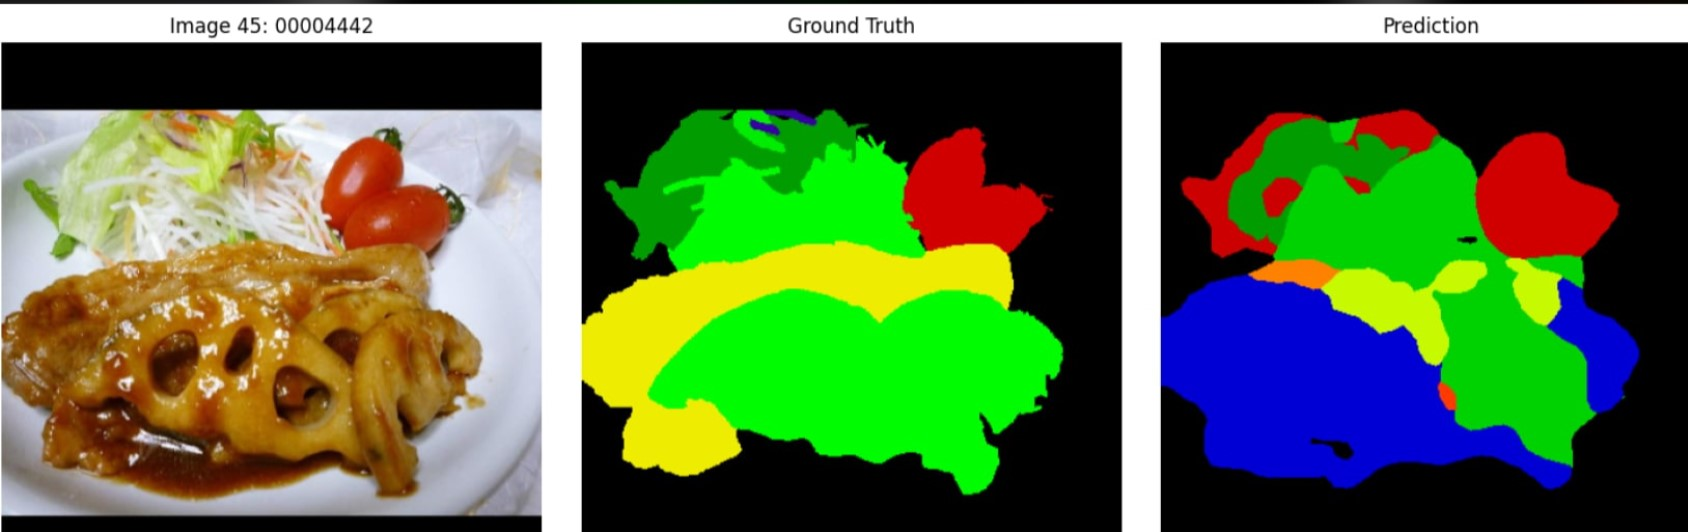
\includegraphics[width=\linewidth]{img/outputs/predict-problem.jpg}
    \caption{Ví dụ lỗi dự đoán điển hình của BiSeNet khi các thành phần nguyên liệu có ranh giới mờ hoặc chồng lấp mạnh.}
    \label{fig:bisenet-predict-problem}
\end{figure}

% Bảng 2: Kết quả đánh giá tổng thể
\begin{table}[H]
    \centering
    \caption{Các chỉ số đánh giá của mô hình cơ sở BiSeNet trên tập kiểm định của bộ dữ liệu FoodSeg103.}
    \label{tab:bisenet-baseline-results}
    \footnotesize
    \begin{tabular}{lc}
        \toprule
        \textbf{Chỉ số} & \textbf{Giá trị} \\
        \midrule
        mIoU & 31.0\% \\
        mAcc & 35.8\% \\
        aAcc & 71.9\% \\
        \bottomrule
    \end{tabular}
\end{table}

Theo tiêu chí đã định nghĩa ở phần trước, \textbf{mIoU} vẫn là chỉ số đánh giá chính vì phản ánh trực tiếp mức giao nhau trên hợp giữa vùng dự đoán và ground truth ở cấp độ pixel. Kết quả trên tập kiểm định cho thấy mô hình đạt $\mathrm{mIoU}=0.31$, $\mathrm{mAcc}=0.41$ và $\mathrm{aAcc}=0.79$. So sánh tương quan giữa ba chỉ số cho thấy độ chính xác toàn cục vẫn cao hơn đáng kể so với các chỉ số trung bình theo lớp, phản ánh tác động của mất cân bằng lớp trong dữ liệu phân đoạn thực phẩm và dư địa cải thiện ở các lớp khó/hiếm.

